\documentclass[abstracton,12pt]{scrreprt}

\usepackage[utf8]{inputenc}
\usepackage[T1]{fontenc}
\usepackage{fancyhdr}
\usepackage{graphicx}
\usepackage{tikz}
\usepackage{times}
\usepackage{listings}
\usepackage{amssymb}
\usepackage{amsfonts}
\usepackage{amsmath}
\usepackage[
backend=bibtex,
style=alphabetic,
]{biblatex}

\addbibresource{bib.bib}


% --------- 

\titlehead{Department of Informatics, University of Zürich}
\subject{\vspace*{2cm}MSc Thesis}
\title{CAVIER}
\subtitle{Cascading View Trees}
\author{
  Johann Schwabe\\[-5pt]
  \scriptsize Matrikelnummer: 17-726-274\\[-5pt]
  \scriptsize Email: \texttt{johann.schwabe@uzh.ch}
}
\date{\vspace*{2cm}08.04.2023}
\publishers{
  \small supervised by Prof.\ Dr.\ D.\ Olteanu and Dr. H.\ Zhang \\[5cm]
  \begin{tikzpicture}[overlay]
    \node at (-3,-3) {
\includegraphics[height=1.5cm]{IFIlogo}};
    \node at (7,-3) {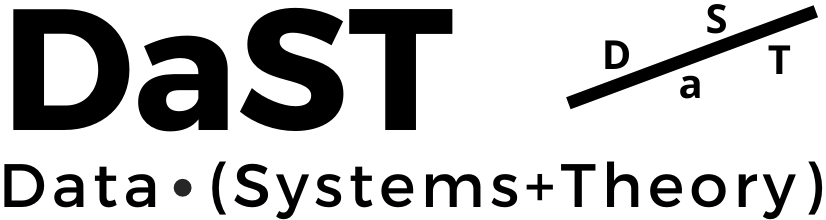
\includegraphics[height=1.5cm]{dast-logo}};
  \end{tikzpicture}
}

\dedication{dedicated to xxx}

% --------- 

\newtheorem{definition}{Definition}
\newtheorem{example}{Example}
\newtheorem{theorem}{Theorem}
\newtheorem{lemma}{Lemma}

\newenvironment{proof}
  {\noindent{\bf Proof:\rm}}{\hfill$\Box$\vspace{\medskipamount}}

\def\bbbr{{\rm I\!R}}
\def\bbbm{{\rm I\!M}}
\def\bbbn{{\rm I\!N}}
\def\bbbz{{\rm I\!Z}}

% --------- 

\begin{document}

\maketitle

\chapter*{Acknowledgements}

\begin{abstract}
  ...
\end{abstract}

\chapter*{Zusammenfassung}

\tableofcontents
\listoffigures
\listoftables

\chapter{Introduction}
Modern databases are under constant change (citetation needed). Thus their underlying database systems must efficiently handle these additions and deletions of tuple. But they must not only update the underlying data and their indices but also the views, presenting important information computed from the data to the users. As many traditional database systems cannot efficiently maintain these views, systems like FIVM were developped to improve on this. While FIVM can efficiently maintain individual views, every view is maintained individually without reusing shared subqueries between similar views. CAVIER, an extension of FIVM, presented in this thesis removes this limitation by focusing on maintaining a group of views and reusing results from previously computed views. Doing so, CAVIER can achieve asymtotically lower computation time than would be possible when individually maintaining the views using FIVM

\chapter{Foundations}
\subsection{Conjunctive Queries}
Conjunctive Queries are the key operation in any database system. They are joins over equality conditions. 
\section{Views and Database Updates}

Databases have to be updated upon tuple additions and deletions. Thus Views need to be updated also. Recomputing is slow. -> Incremental updates

\section{Factorized Databases}
Factorized Databases are an alternative form of representing tuples in a relation. Traditional databases save a list of tuples for each relation and compute the join over them on demand, returning again lists of tuples. Contrary, Factorized Databases decompose the relations, for each query to a tree using laws of relational algebra. Using the law of distributivity of the Cartesian Product over unions much of the redundant information within the traditional listing representation can be removed. Thus they are a succient and lossless compression of the data for a given query. As the tuples aren't explicitly listed, they have be enumerated and the enumeration time is dependant of the variable order and thus the query. 
The example from \cite{FactorizedDB} (Figure \ref{fig:factorizedDBExample}) highlights the advantages well: While the listed result of the natural join of \textbf{Sales, Branch, Competition} uses 90 values, the factorized relation can compress the result to 20 values. Factorized databases aren't limited to joins but also support aggregation and group by clauses and can thus be used for most modern SQL queries.
The main drawback of factorized databases is that for each query a variable order needs to be found and for this variable order a Factorized representation built. Finding a good variable order is crucial to achieving a succient representation and thus efficient enumeration. \cite{FactorizedDB}
\begin{figure}
	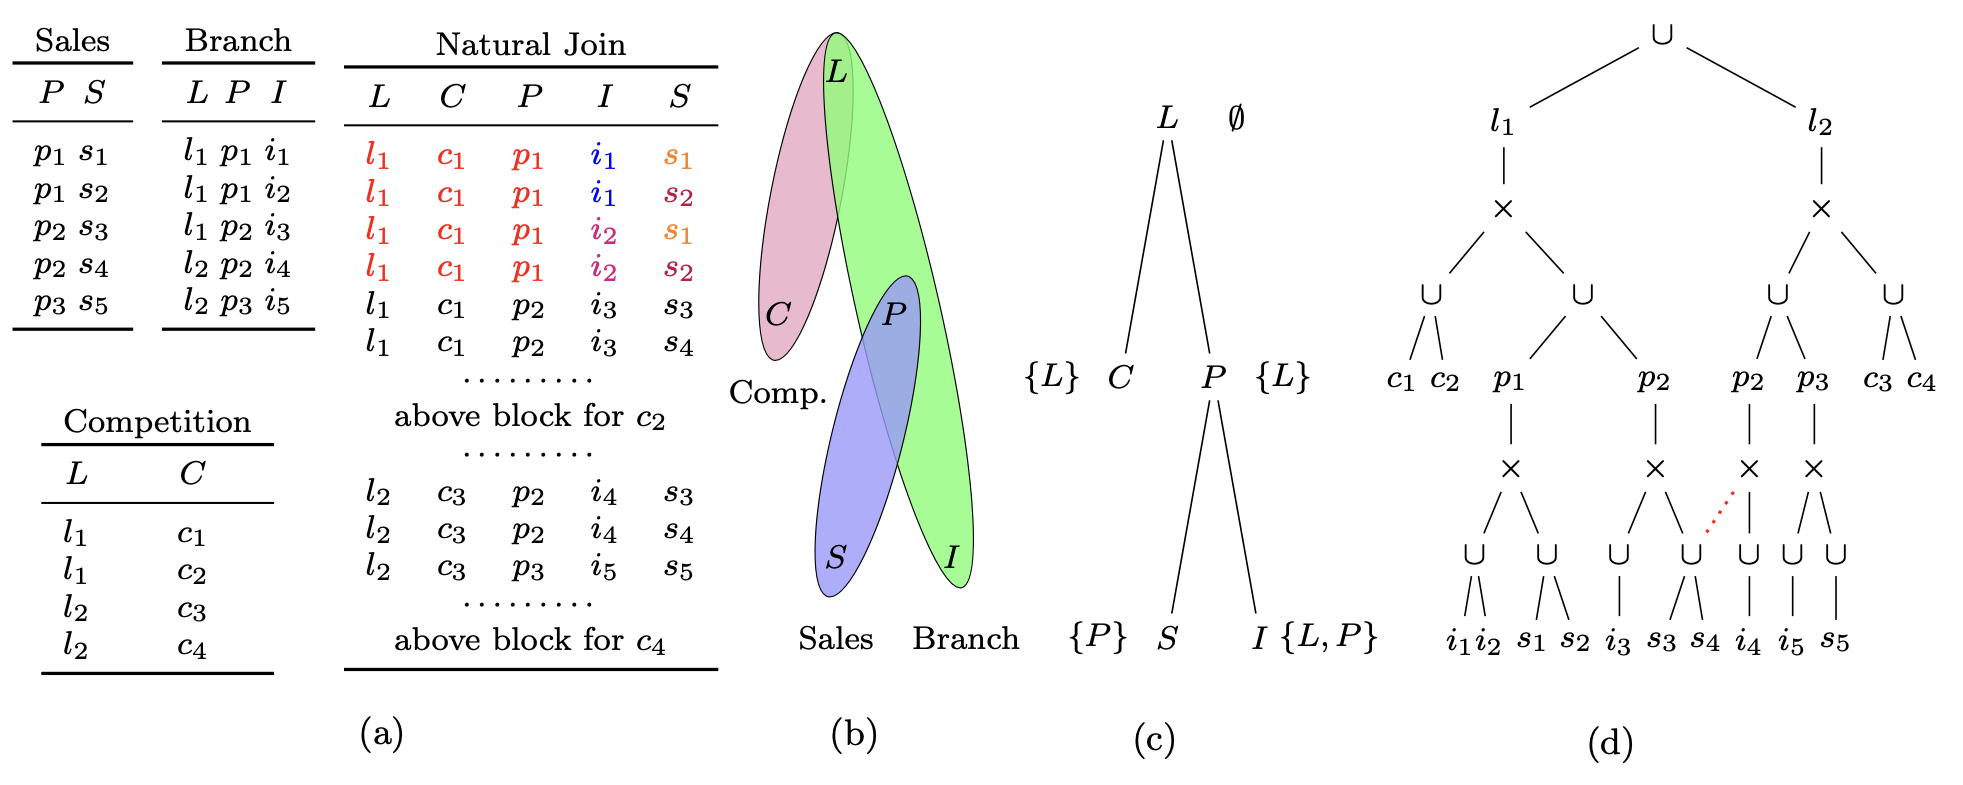
\includegraphics[width=\linewidth]{FactorizedExample.png}
	\caption{An example of a Factorized Database: a) Listing Representation, b) Hypergraph of the join, c) Variable order, d) Factorized Representation \cite{FactorizedDB}}
	\label{fig:factorizedDBExample}
\end{figure}


\subsection{Preprocesing vs enumeration vs update time}
Three key timeconsuming aspects

\subsection{Q-hierarchical}
very nice
O(1) $\And$ O(1) $\And$ O(1)

\subsection{FIVM}
\subsection{DB-Toaster}

\chapter{Results}
\section{Cavier}
\subsection{Algorithm}
\subsection{Improvements}
\subsection{Limitations}
\subsection{Extensions}
\section{Benchmarks}

\chapter{Discussion}

\chapter{Conclusion}

\chapter{Appendix}

\printbibliography


\end{document}
